\documentclass{beamer}
\usepackage{beamerthemesplit} 
\usepackage{tikz}
\usetikzlibrary{trees}


\title{Computational Physics Group Project: \\ Ecosystem: predator and prey}
\author{David Hicks\\ Weiyao Ke \\ Shagun Maheshwari \\ Fan Zhang}
\date{\today}

\begin{document}

\frame{\titlepage}

\section[Outline]{}
\frame{\tableofcontents}

\section{Introduction to eco-system modelling}

\frame
{
	\frametitle{Population interaction of predator and prey in eco-system}

	\begin{figure}[htbp]
	\begin{center}
	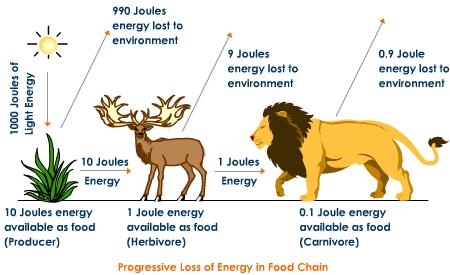
\includegraphics[width=0.6\textwidth]{./pics/progressive-energy-loss.jpeg}
	\caption{default}
	\label{default}
	\end{center}
	\end{figure}
}


\frame
{
 	\frametitle{Population interaction of predator and prey in eco-system}
 
	\begin{figure}[htbp]
	\begin{center}
		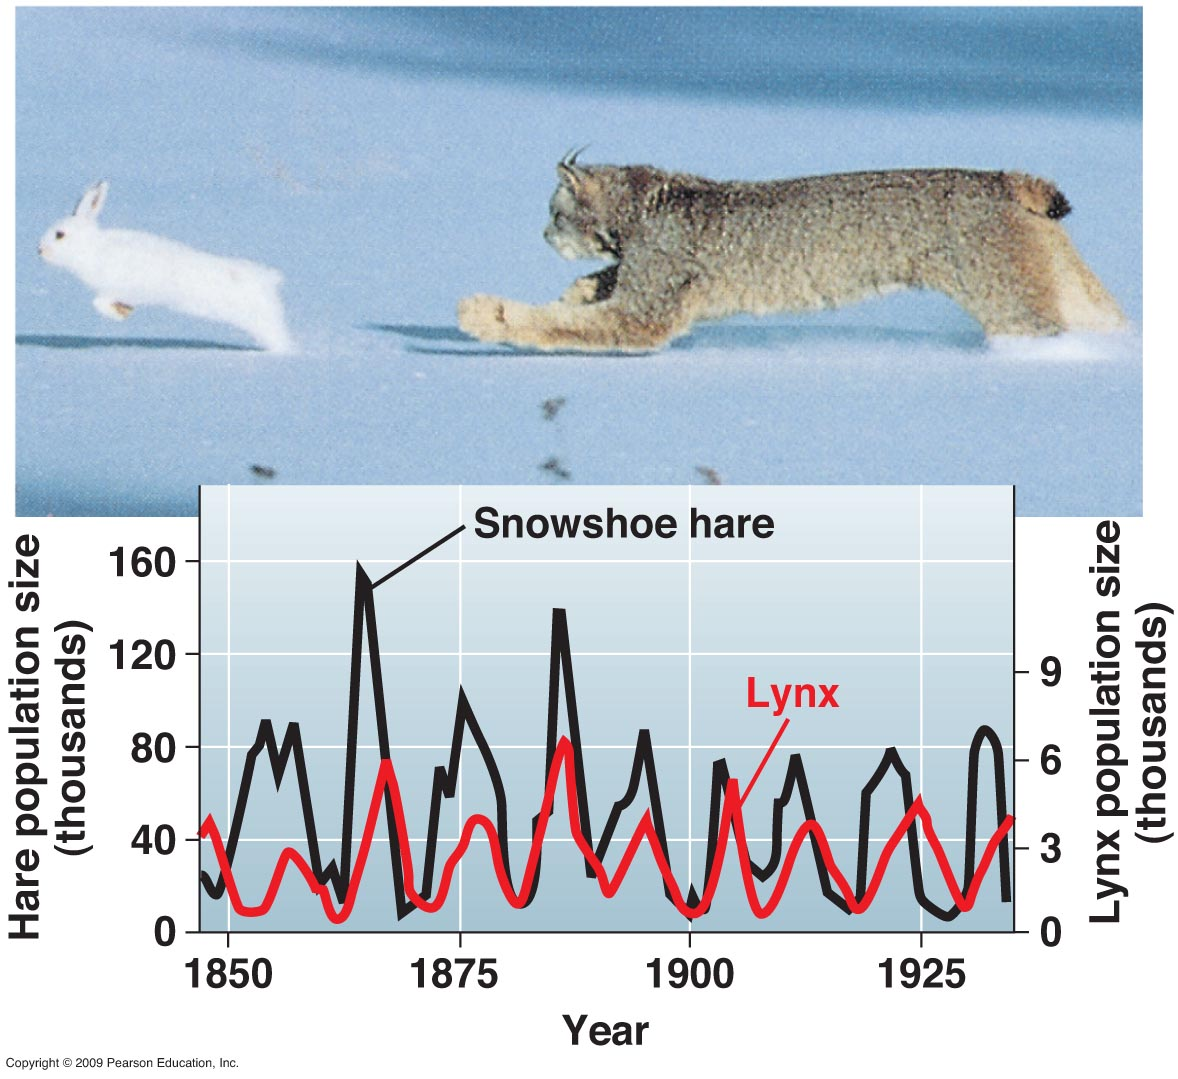
\includegraphics[width=0.4\textwidth]{./pics/predator_prey2.jpeg}
	\caption{http://www.anselm.edu/homepage/jpitocch/genbi101/ecology1intropops.html}
	\label{default}
	\end{center}
	\end{figure}  
}

\frame
{
 	\frametitle{A simplified determinsitic mode: L-V equation}

}


\frame
{
  \frametitle{Simulation of a eco-system with predator and prey}
  A simulation keep the essential nature of the interaction between and within the species, and predict the evolution of population step by step.
  \begin{itemize}
  \item<1->{Both predator and prey reproduces when they reach the age of reproduction}
  \item<2->{Predator feeds on prey.}
  \item<3->{Predator and prey will die out if maximum age is reached or starved for enough long time}
  \item<4->{However, simulation is a random process and change the deterministic nature of LV equation (more realistic).}
  \end{itemize} 
}

\section{Implementation of the simulation}
\frame
{
  \frametitle{Structural setup}

\tikzstyle{every node}=[anchor=west]
\begin{tikzpicture}
[grow via three points={one child at (0.5,-0.5) and two children at (0.5,-0.5) and (0.5,-1)}, edge from parent path={(\tikzparentnode.south) |- (\tikzchildnode.west)}]
  \node {Animal Class $\rightarrow$ Deer/ Wolf}
    child{ node{variables}
    	     	child { node {presentation position}}		
   		child { node {previous position}}
    		child { node {reproducing age variable}}
    		child { node {starving age variable}}
    	}
    child [missing] {}				
    child [missing] {}				
    child [missing] {}	
    child [missing] {}	
    child{ node{constants}
    		child { node {starvation age}}
    		child { node {reproduction age}}
	}
    child [missing] {}	
    child [missing] {}	
    child{ node{functions}
    		child { node {check status: live/dead}}
    		child { node {check maturity: procreate/not}}
	};		
\end{tikzpicture}
}

\frame
{
  \frametitle{Structural setup}

\tikzstyle{every node}=[anchor=west]
\begin{tikzpicture}
[grow via three points={one child at (0.5,-0.5) and two children at (0.5,-0.5) and (0.5,-1)}, edge from parent path={(\tikzparentnode.south) |- (\tikzchildnode.west)}]
  \node {Eco-system}
    child{ node{variables}
    	     	child { node {a list of deer}}		
   		child { node {a list of wolves}}
		child { node {occupation matrix (0, 1, 2) $\rightarrow$ (vacant, deer, woof)}}
    		child { node {system time}}
    	}
    child [missing] {}				
    child [missing] {}				
    child [missing] {}	
    child [missing] {}
    child{ node{constants}
    		child { node {Initialisation parameters: world size, starvation ages}}
	}
    child [missing] {}	
    child{ node{functions}
    		child { node {initialisation}}
    		child { node {time evolution}}
	};		
\end{tikzpicture}
}


\frame
{
  \frametitle{Initialisation}
  A sanity simulation requires several constrains on the initialisation of parameters.
  \begin{itemize}
  \item<1->{Reproduction age of predators must be larger than their starvation age. (Or else wolf can sustain themselves ...)}
  \item<2->{Starvation age of the deer is extremely large. (Always enough plants!)}
  \end{itemize} 
}

\frame
{
  \frametitle{time evolution (All things are done serially!)}
  \begin{itemize}
  \item<1->{Step1: loop over wolves and deer and increase ages by 1; then check if they are alive. Only live animals are kept in list for operations below.}
  \item<2->{Step2: loop over wolves and check neighbours. If deer nearby, capture a random one and move to that position. If no deer but vacancies around, move to a random location. If a mature wolf's present location differs from previous location, deposits a new-born at its previous location.} 
  \item<3->{Step3: loop over deer and delete those whose location are now occupied by wolves (via the occupation matrix)}
  \item<4->{Step4: loop over deer and check neighbours. If vacancies around, move to a random location. If a mature deer's present location differs from previous location, deposits a new-born at its previous location.} 
  \item<5->{Step5: go back to Step1 and increase system time by 1}
  \end{itemize} 
  
}
\frame
{
  \frametitle{Simulation of a eco-system with predator and prey}
  %Add what you want here
  We set up a $N \times N$ grid and simulate the eco-system with L-V equation. \\
  Evolution Step $1$: check wolf and deer population, increase its age, and see whether a single animal has starved to death. \\
  Evolution step $2$: evolution of wolves: \\
  \begin{figure}[htb]
  \begin{center}
  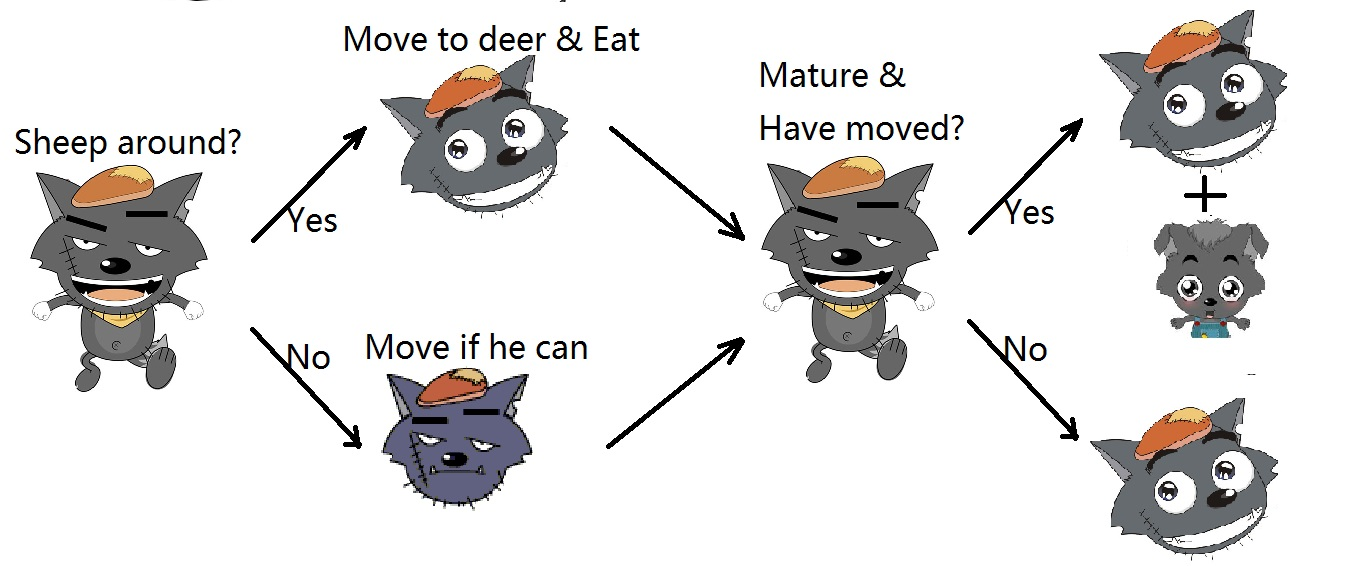
\includegraphics[width=\textwidth]{wolf.jpg}
  \label{default}
  \end{center}
  \end{figure}
}
\frame
{
  \frametitle{Evolution step 3}
  Evolution of deers: \\
  \begin{itemize}
  \item 1. Delete all unfortunate deers. \\
  \pause
  \item 2. Evolution of live deers. \\
  \end{itemize}
  \begin{figure}[htbp]
  \begin{center}
  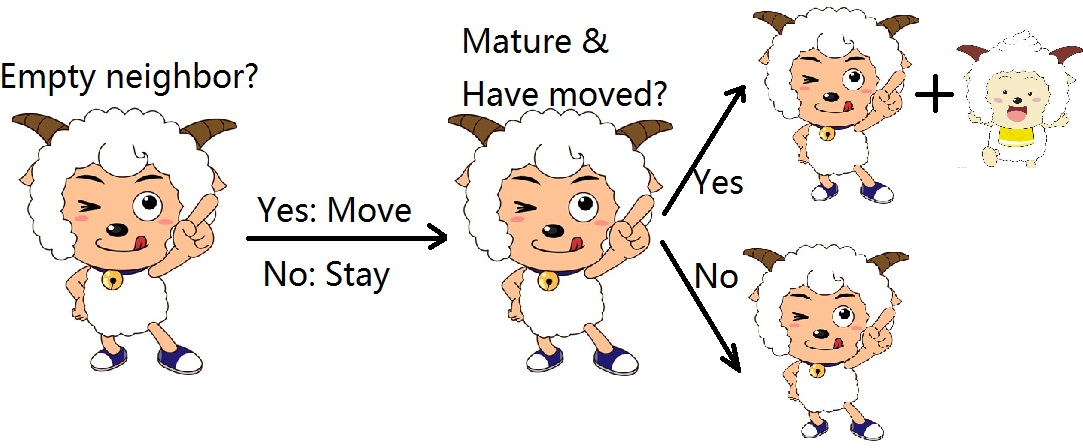
\includegraphics[width=\textwidth]{goat.jpg}
  \label{default}
  \end{center}
  \end{figure}
}
\frame
{
  \frametitle{parameter scanning}
  %Add what you want here
  
}

\frame
{
  \frametitle{Parameter Search}
  \underline{5 parameters to test (5-D parameter space)}
  \begin{itemize}
  \item{\textbf{Initial population of deer}}
  \item{\textbf{Initial population of wolves}}
  \item{Reproduction age of deer}
  \item{Reproduction age of wolf}
  \item{Starvation "age" of wolf}
  \end{itemize} 

  \underline{Reduce to 4 dimensions (4-D)}
  \begin{itemize}
  \item{\textbf{Ratio of initial populations : Size of point}}
  \item{Reproduction age of deer : x-axis}
  \item{Reproduction age of wolf : y-axis}
  \item{Starvation "age" of wolf : z-axis}
  \end{itemize} 

}
\frame
{
  \frametitle{Results of Full Parameter Search}
  \begin{figure}[H]
  \centering
        \begin{tabular}{@{}cc@{}cc@{}cc@{}}
                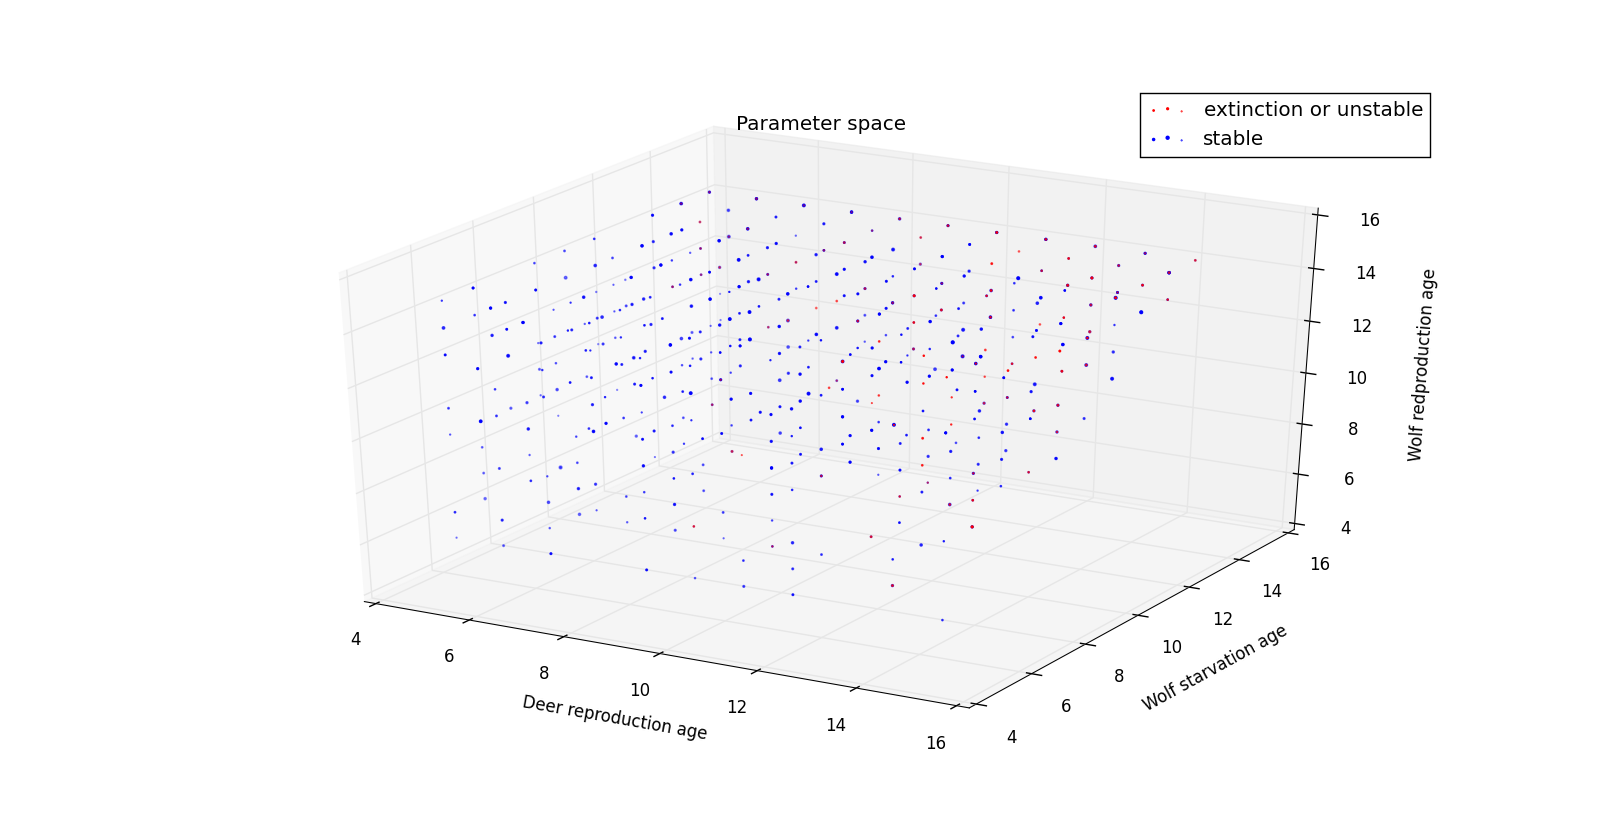
\includegraphics[width = 0.3\textwidth]{./pics/Eco_All_param_front.png} \\
                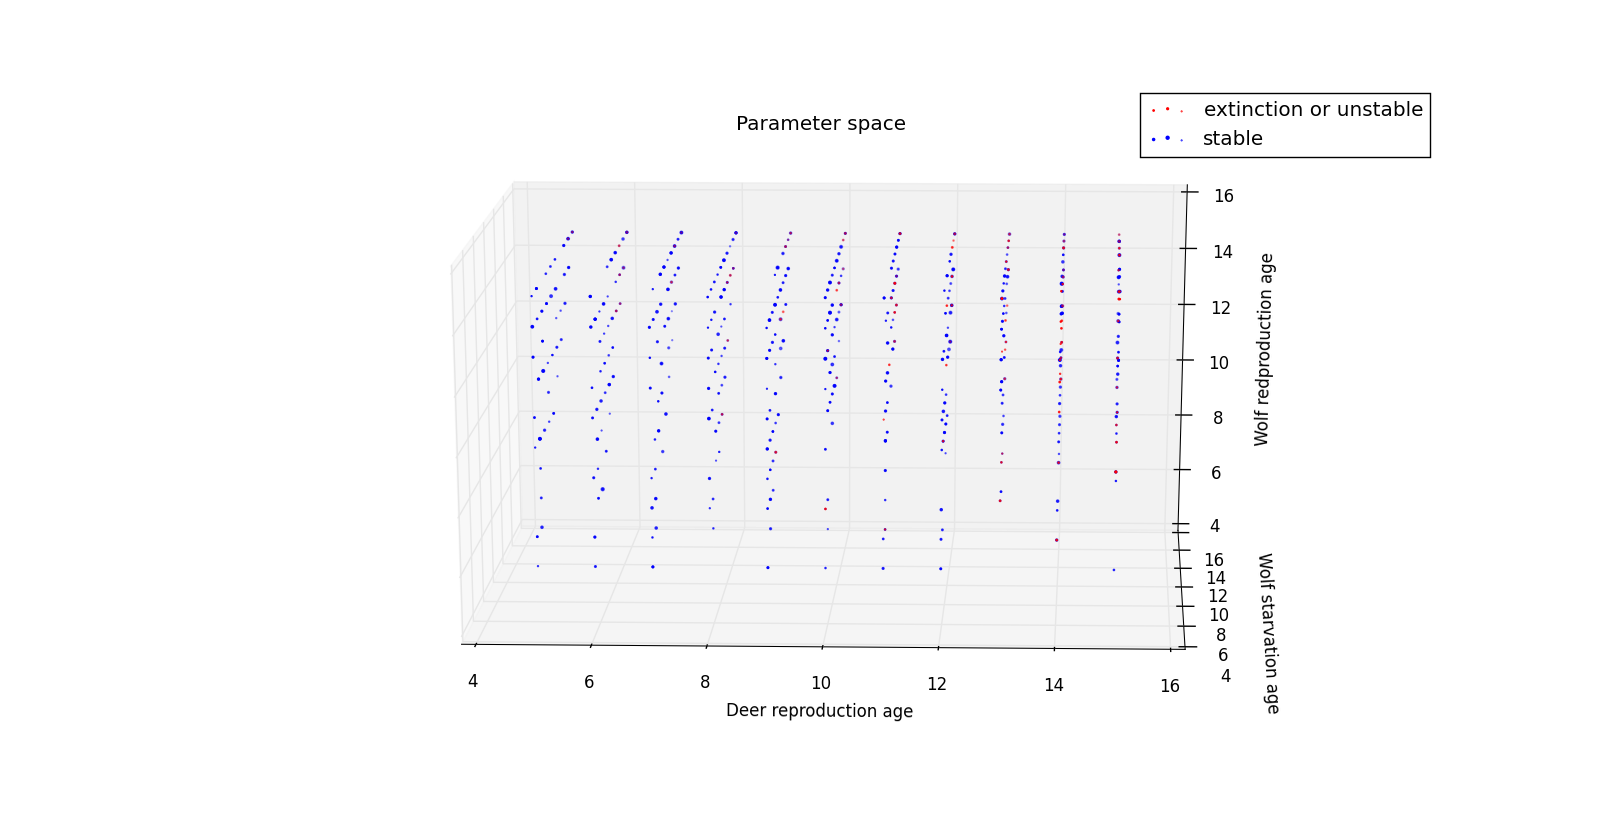
\includegraphics[width = 0.3\textwidth]{./pics/Eco_All_param_rep_v_rep.png} &&
                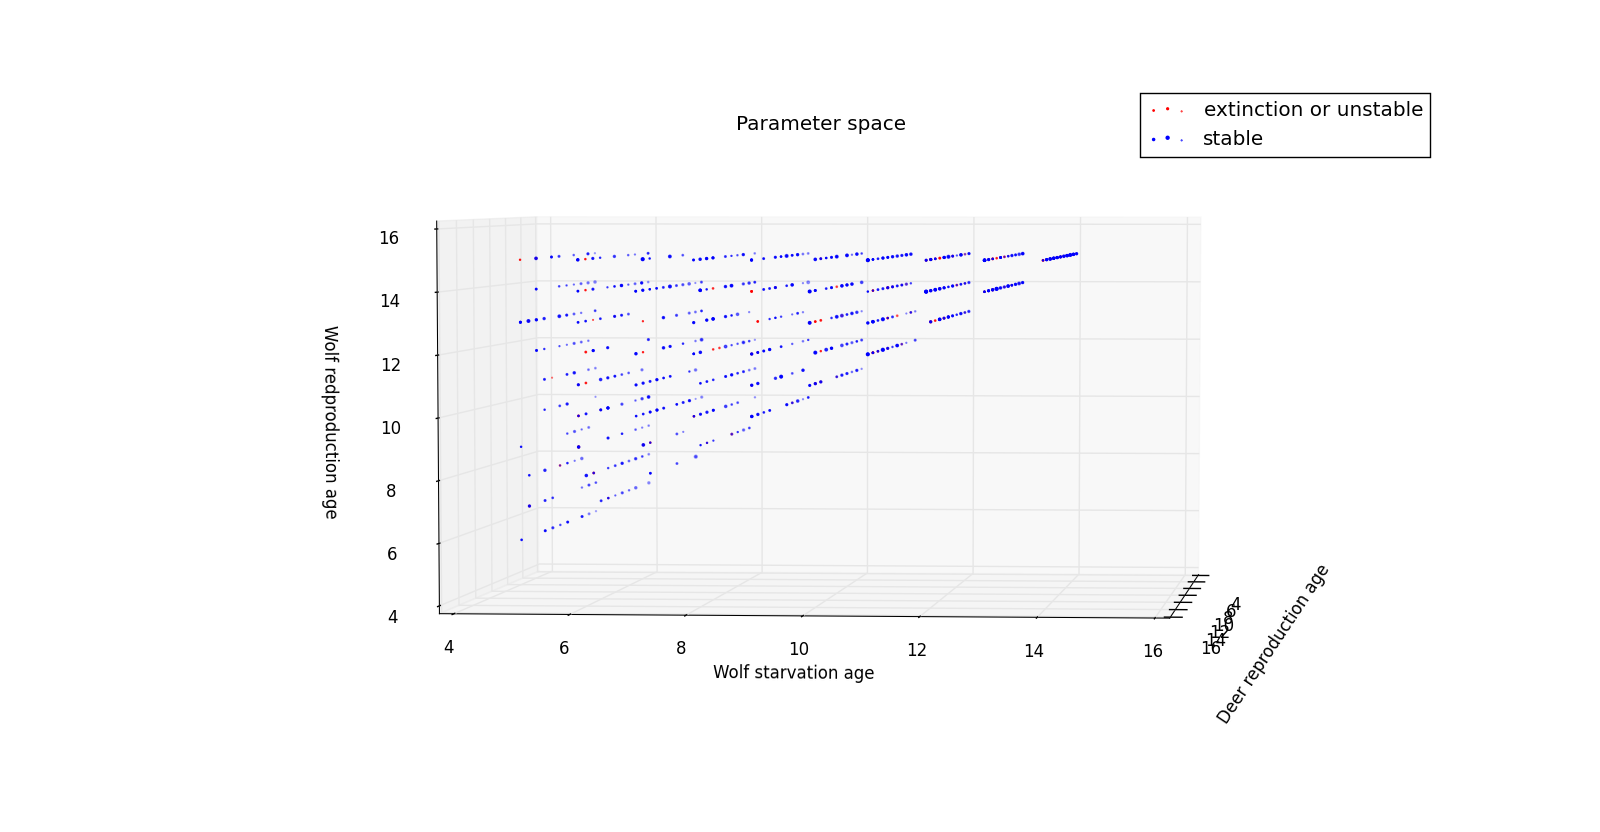
\includegraphics[width = 0.3\textwidth]{./pics/Eco_All_param_wage_v_wstarve.png} &&
                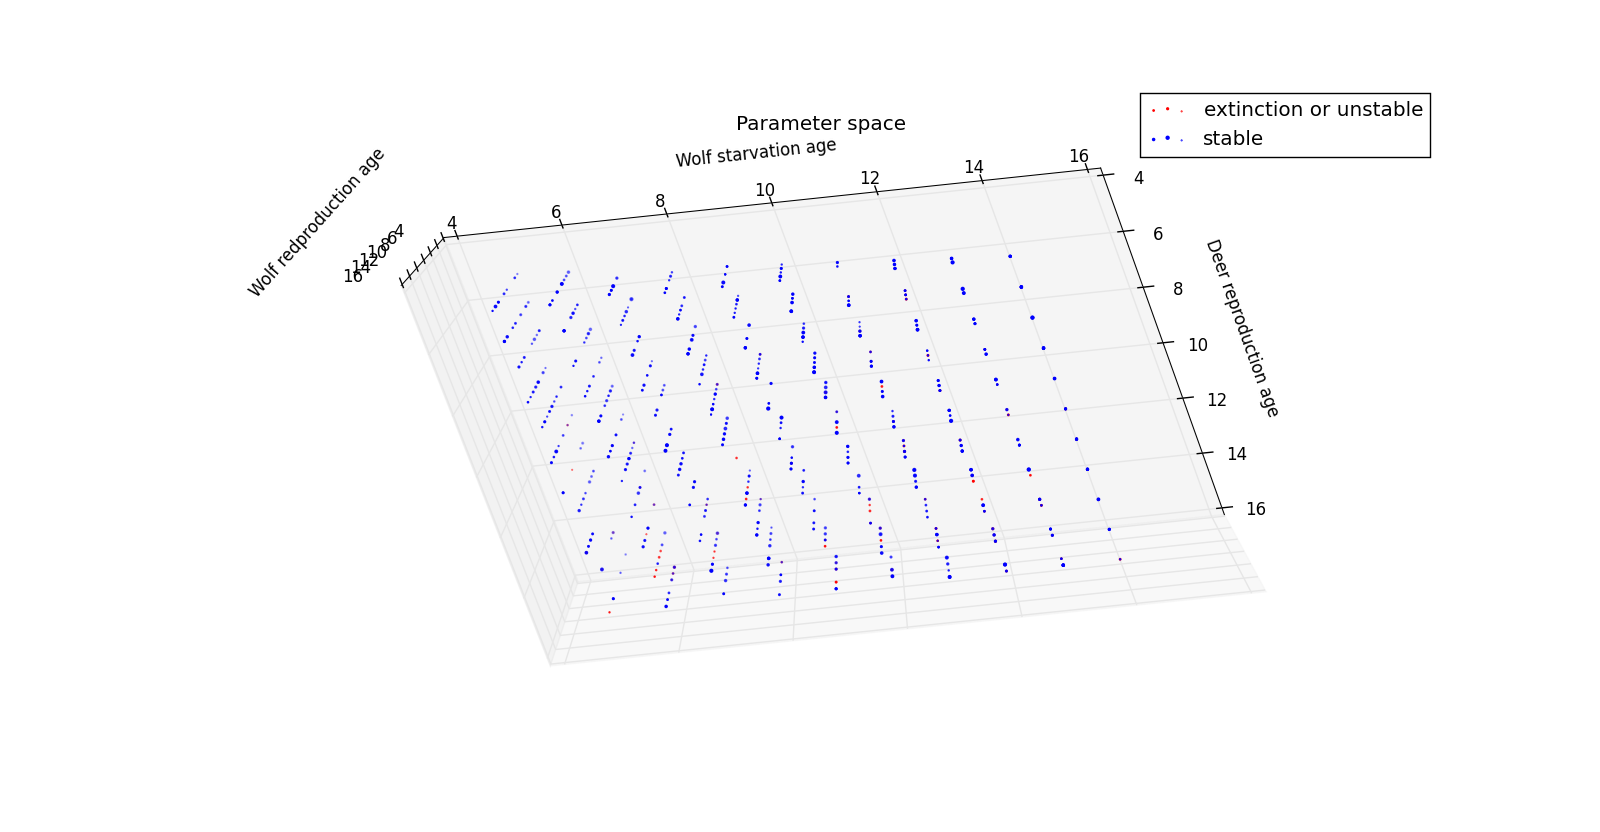
\includegraphics[width = 0.3\textwidth]{./pics/Eco_All_param_wstarve_v_drep.png} \\
        \end{tabular}
        \label{RestrictParam}
  \end{figure}

}

\frame
{
  \frametitle{Results of Restricted Parameter Search}
  \center{Fix initial population ratios}
  \begin{figure}[H]
  \centering
        \begin{tabular}{@{}cc@{}cc@{}}
                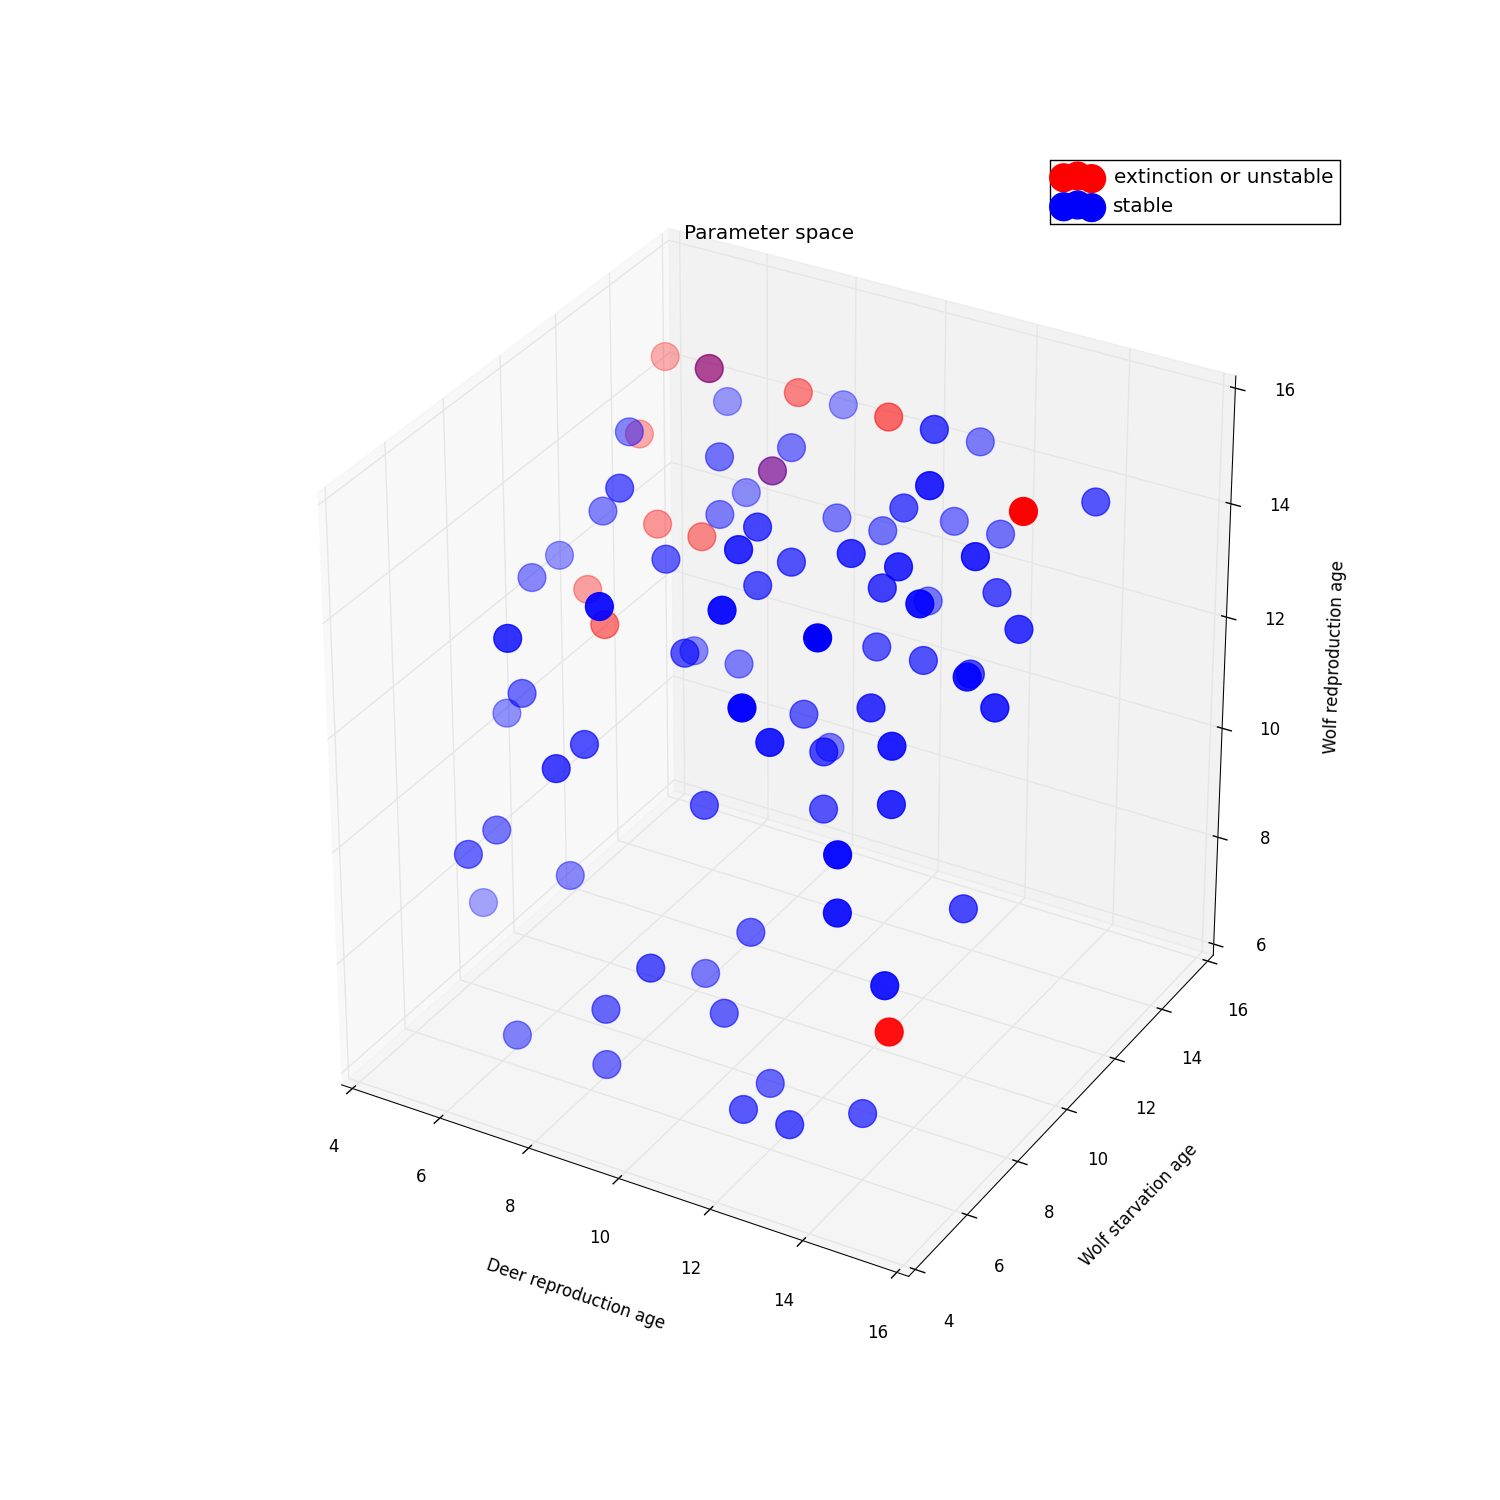
\includegraphics[width = 0.3\textwidth]{./pics/Restricted_Parameter_space_d2500_w250.png} &
                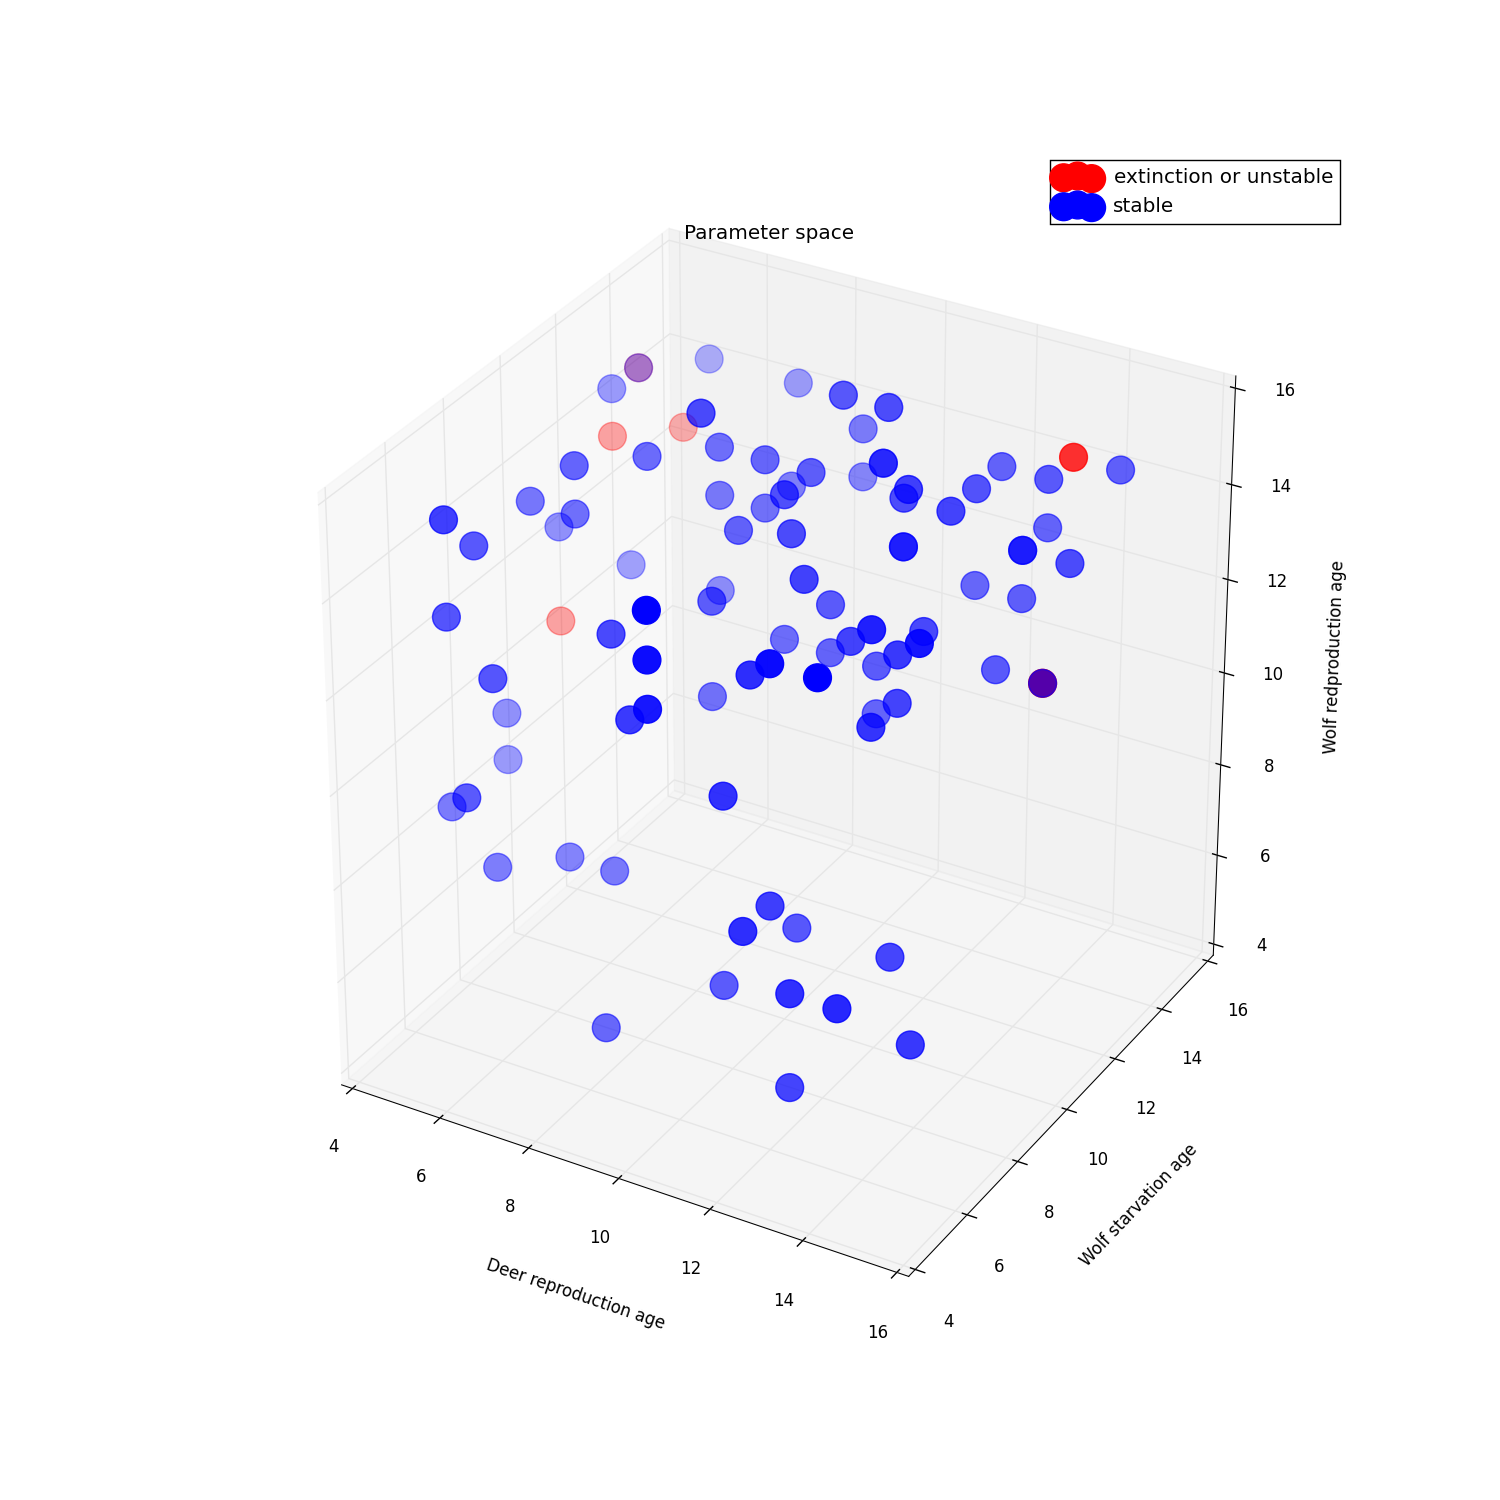
\includegraphics[width = 0.3\textwidth]{./pics/Restricted_Parameter_space_d3000_w500.png} &
                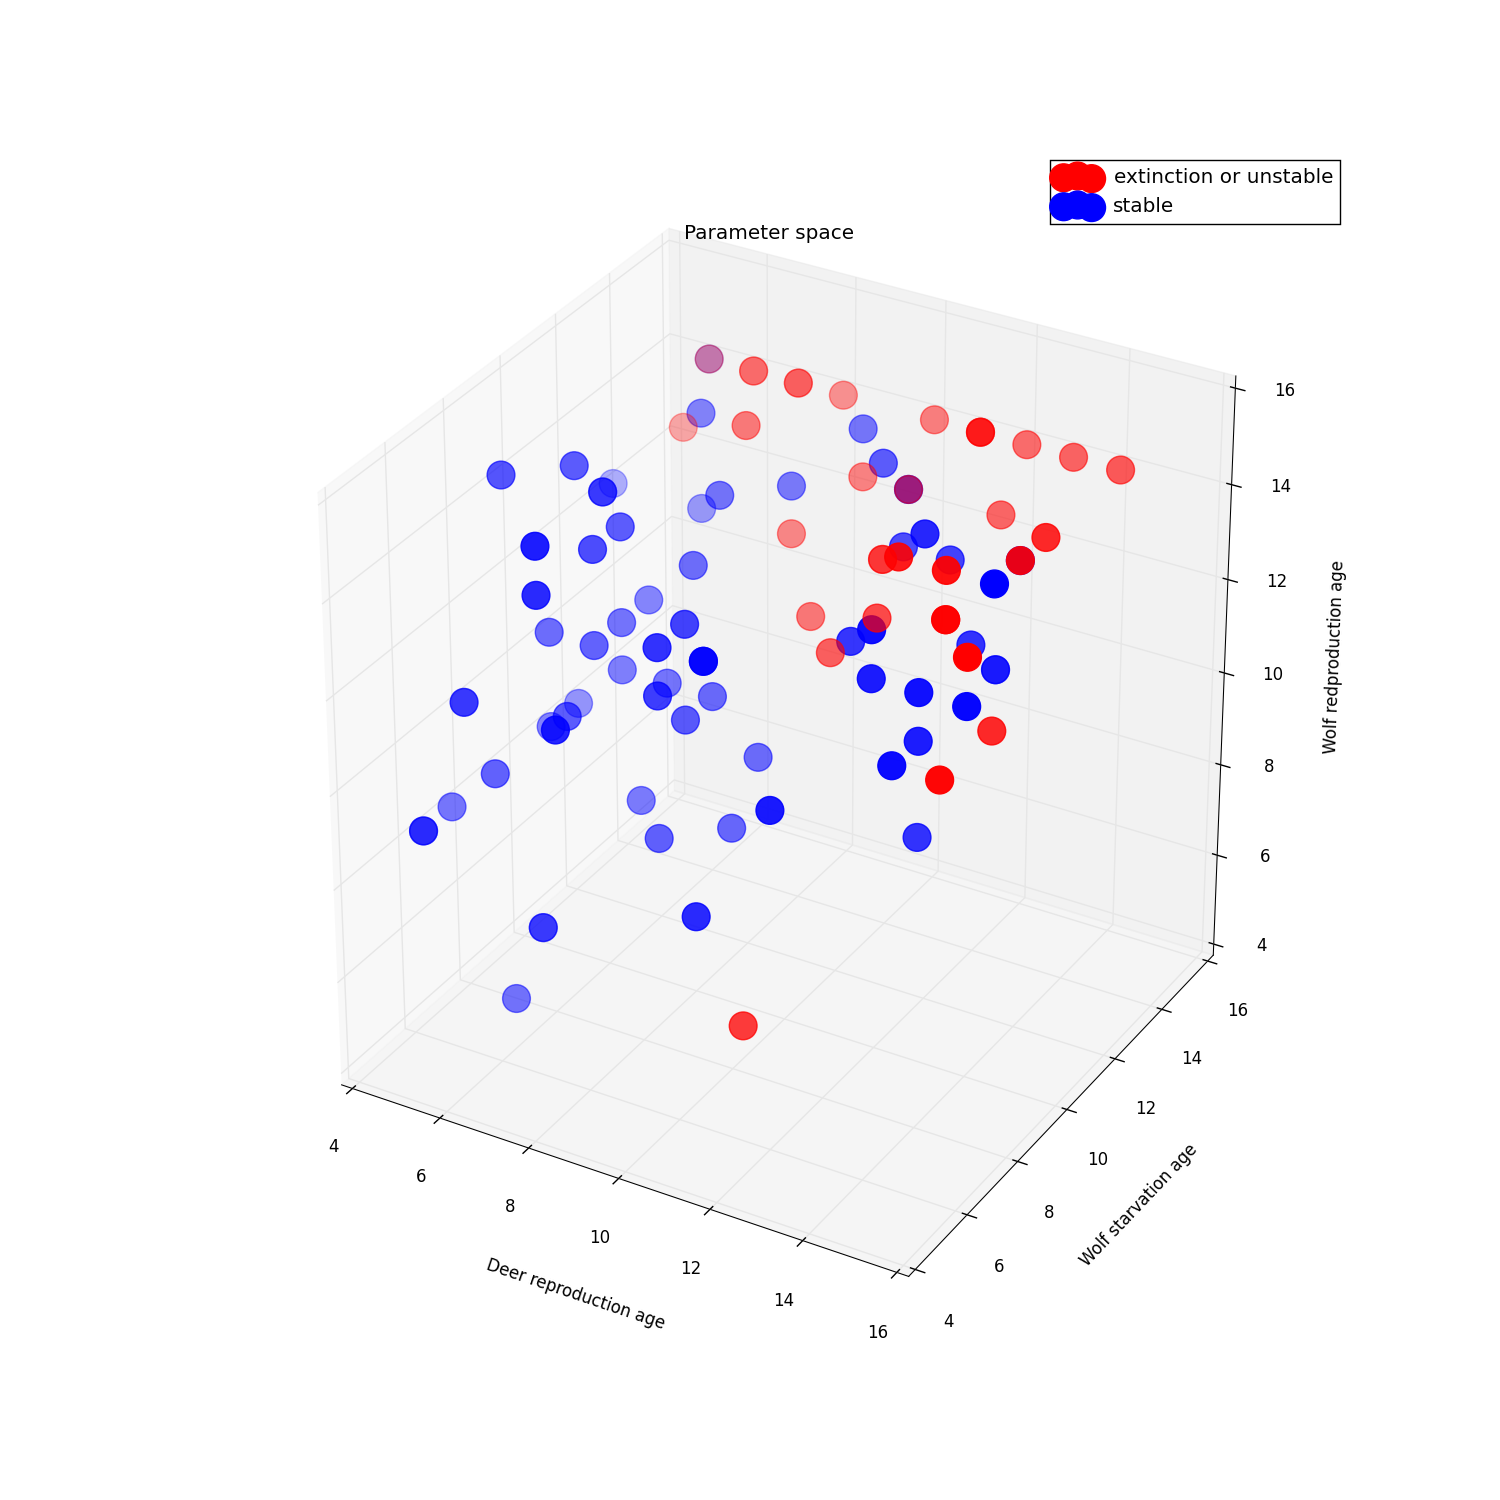
\includegraphics[width = 0.3\textwidth]{./pics/Restricted_Parameter_space_d2000_w2000.png} \\
                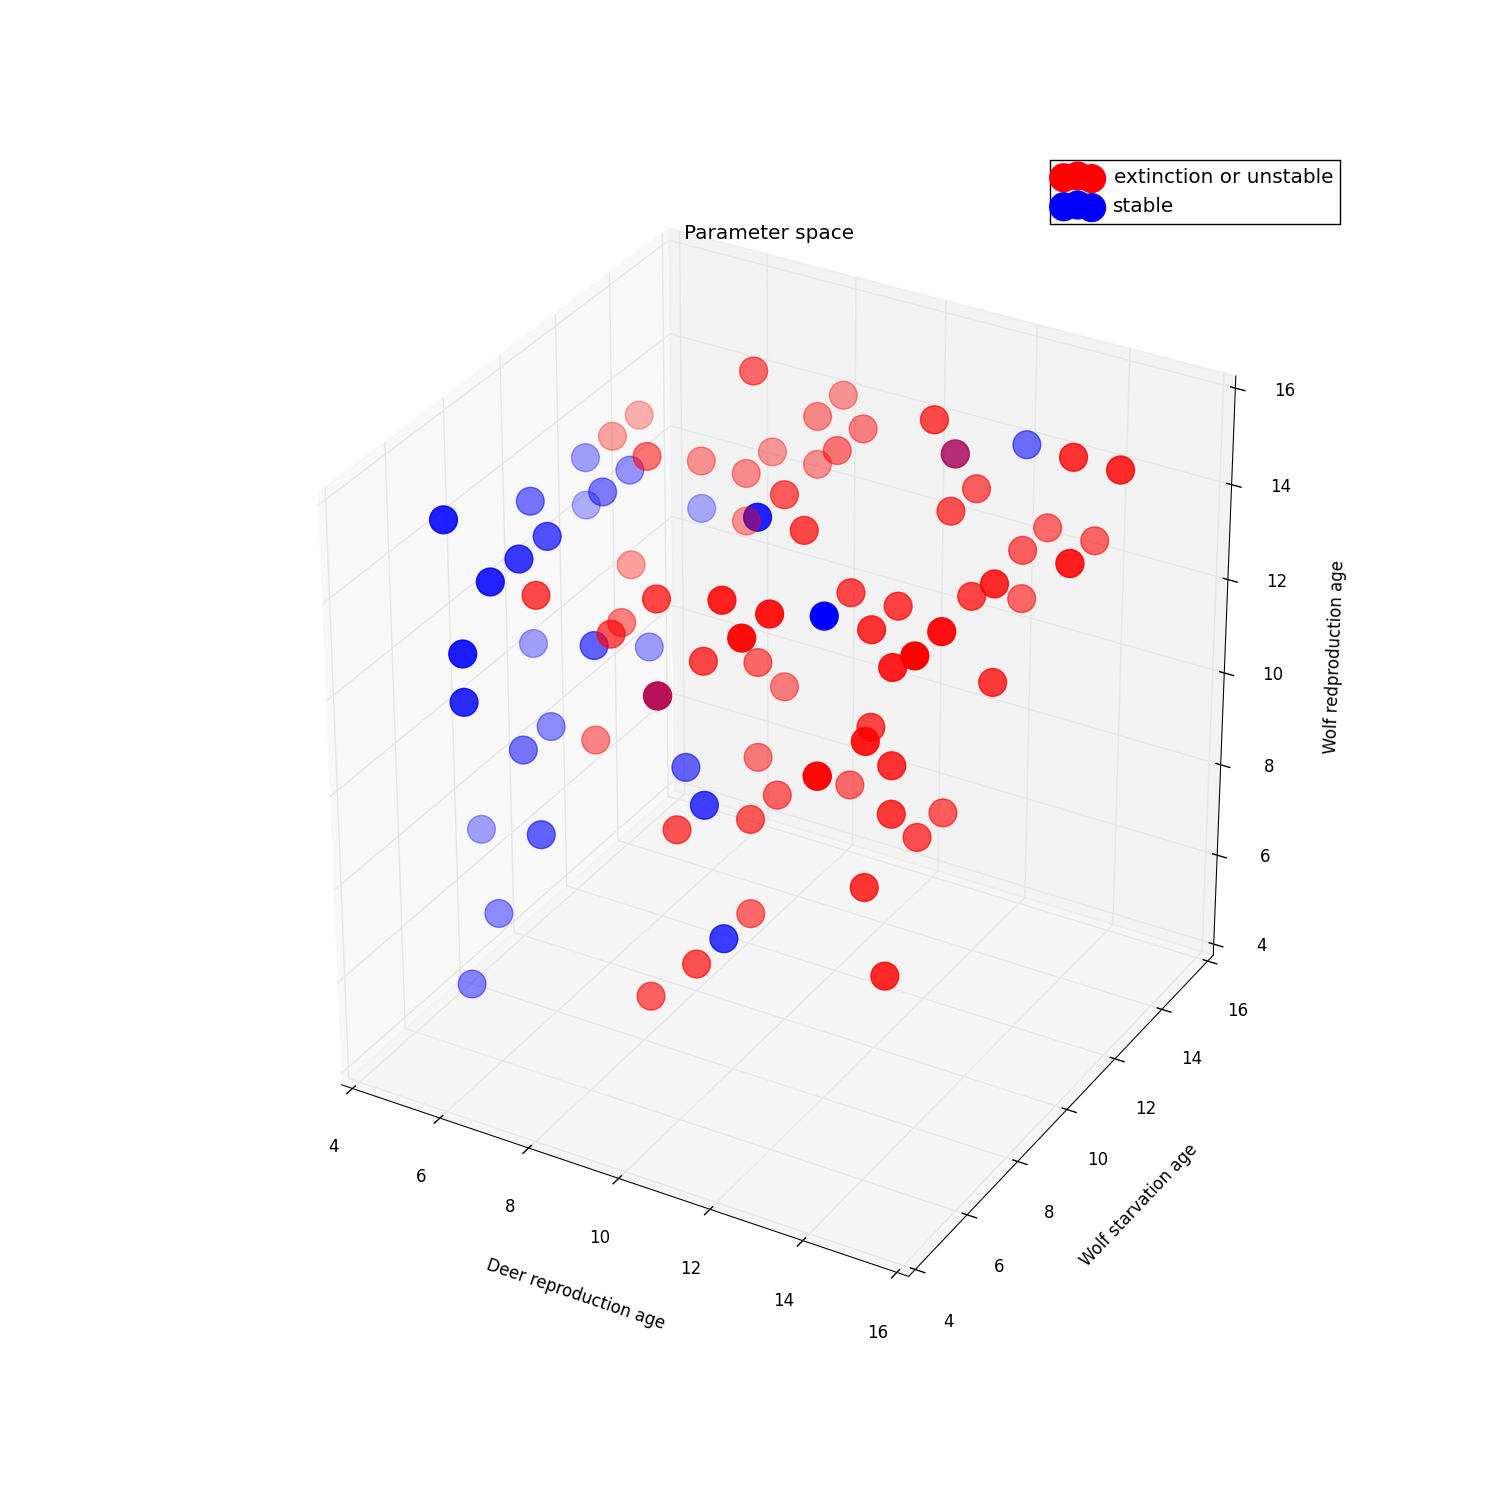
\includegraphics[width = 0.3\textwidth]{./pics/Restricted_Parameter_space_d500_w3000.png} &&
		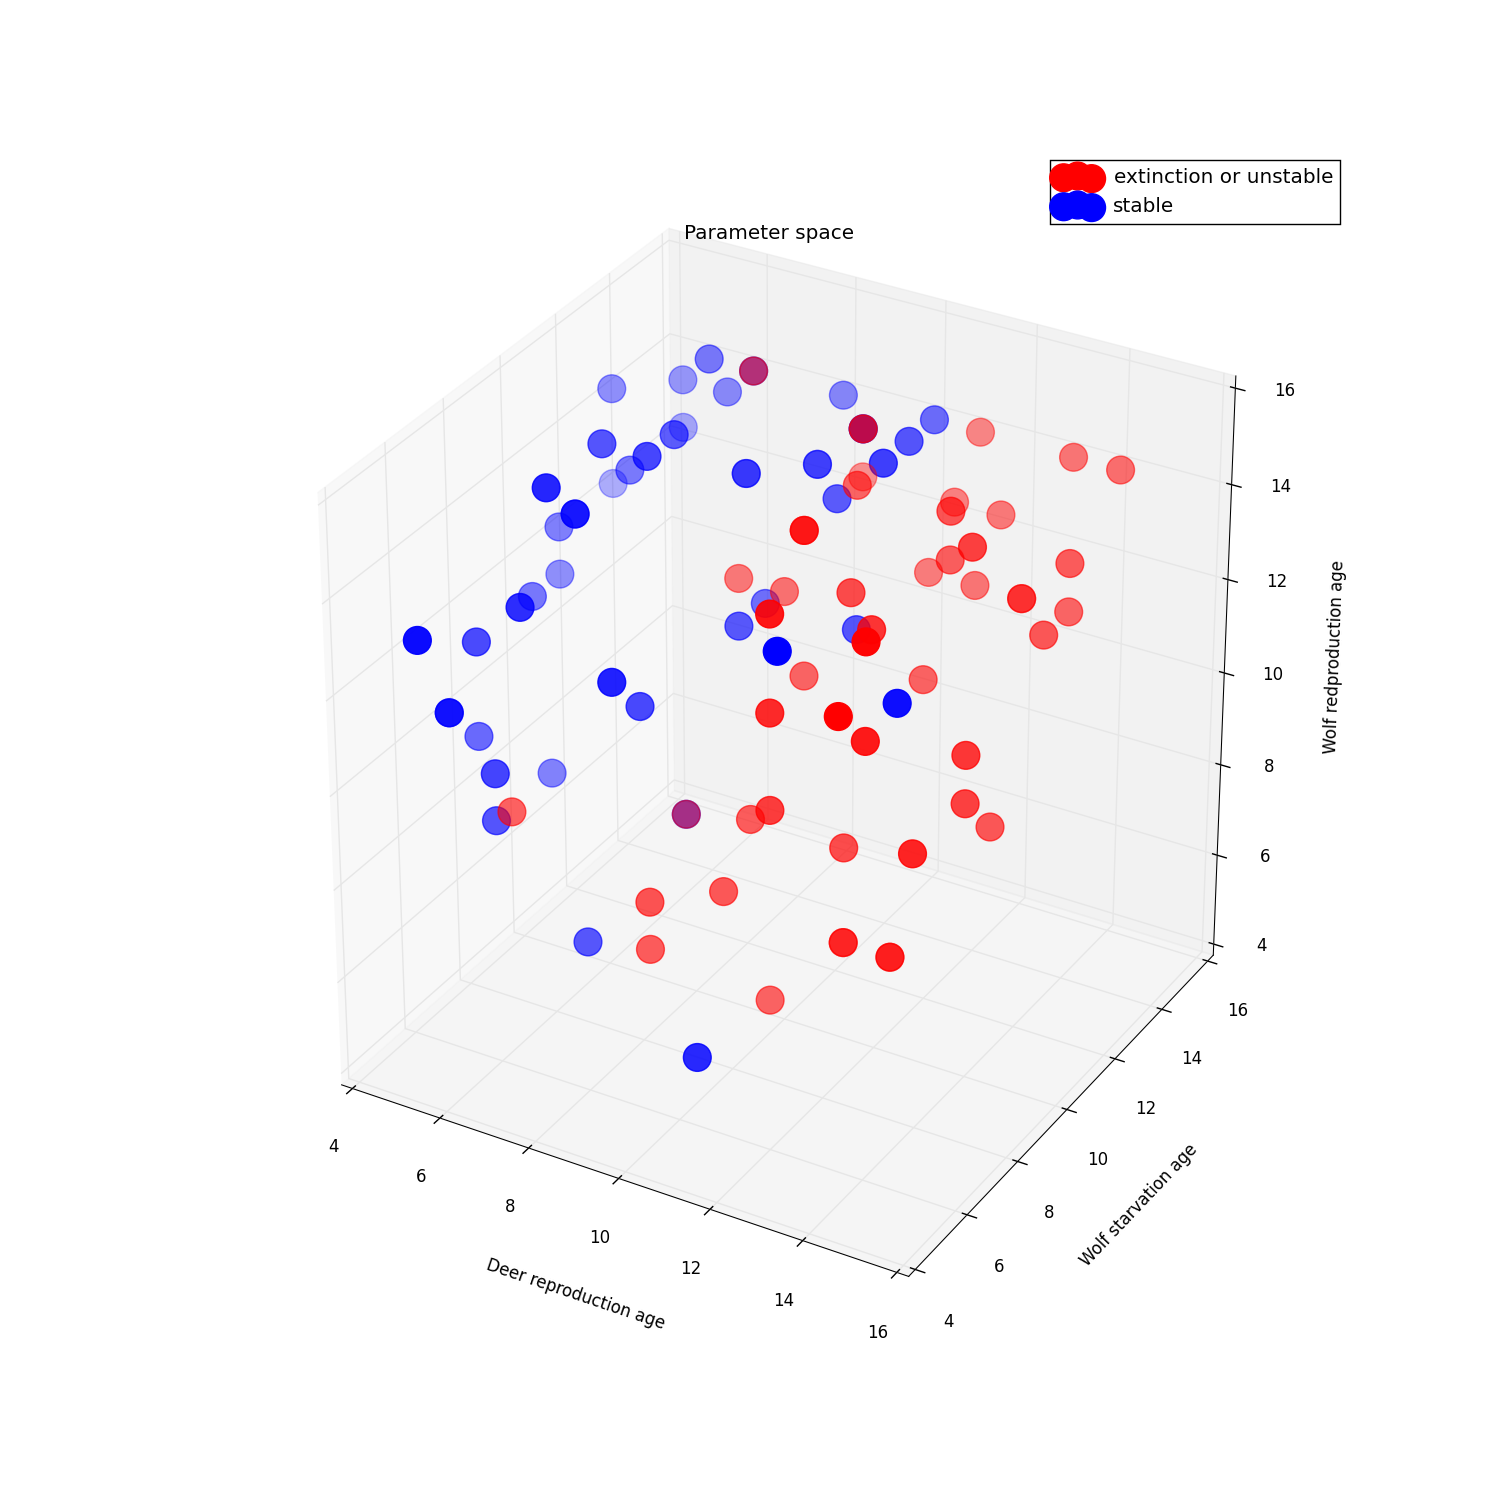
\includegraphics[width = 0.3\textwidth]{./pics/Restricted_Parameter_space_d250_w2500.png} \\
        \end{tabular}
        \label{RestrictParam}
  \end{figure}


}



\section{Results and discussion}
\frame
{
  \frametitle{Ecosystem at Equilibrium}
  Parameters used: 
  \begin{itemize}
  \item{Initial number of deer: 2,500}
  \item{Initial number of wolves: 250}
  \item{Deer reproduction rate: 5}
  \item{Wolf reproduction rate: 14}
  \item{Wolf starvation rate: 11}
  
  \center{ Animation Time! }

  %Add what you want here
  
}


\end{document}
